\chapter{Přílohy}
\pagenumbering{arabic}
\setcounter{page}{1}
\section*{A. Stuktura Operátor SDK projektu\label{atch:tree}}

\begin{figure}[H]
  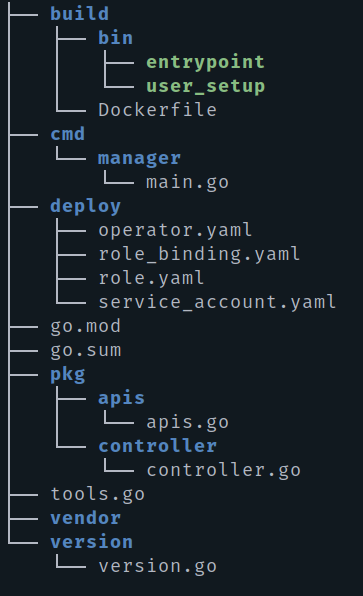
\includegraphics[width=0.5\textwidth]{img/operatorsdk_tree.png}
\end{figure}

\clearpage

\section*{B. Příkazy pro konfiguraci MySQL a RabbitMQ\label{atch:command}}
\begin{verbatim}
// MySQL
CREATE DATABASE cidner;
CREATE DATABASE glance;
CREATE DATABASE keystone;
CREATE DATABASE neutron;
CREATE DATABASE nova;
CREATE DATABASE nova_api;
CREATE DATABASE nova;
CREATE DATABASE nova_cell0;

GRANT ALL PRIVILEGES ON *.* TO 'nova' IDENTIFIED BY 'cloudlab';
GRANT ALL PRIVILEGES ON *.* TO 'nova_cell0' IDENTIFIED BY 'cloudlab';
GRANT ALL PRIVILEGES ON *.* TO 'nova_api' IDENTIFIED BY 'cloudlab';
GRANT ALL PRIVILEGES ON *.* TO 'cinder' IDENTIFIED BY 'cloudlab';
GRANT ALL PRIVILEGES ON *.* TO 'glance' IDENTIFIED BY 'cloudlab';
GRANT ALL PRIVILEGES ON *.* TO 'keystone' IDENTIFIED BY 'cloudlab';
GRANT ALL PRIVILEGES ON *.* TO 'neutron' IDENTIFIED BY 'cloudlab';

//RabbitMQ
rabbitmqctl add_user openstack cloudlab
rabbitmqctl set_user_tags openstack administrator
rabbitmqctl set_permissions -p / openstack ".*" ".*" ".*"
\end{verbatim}

\clearpage